\section {Unpacking}
\label{sec:unpacking}
The \lucid cameras are equiped with a 12-bit \gls{adc}

\begin{figure}
    \centering
    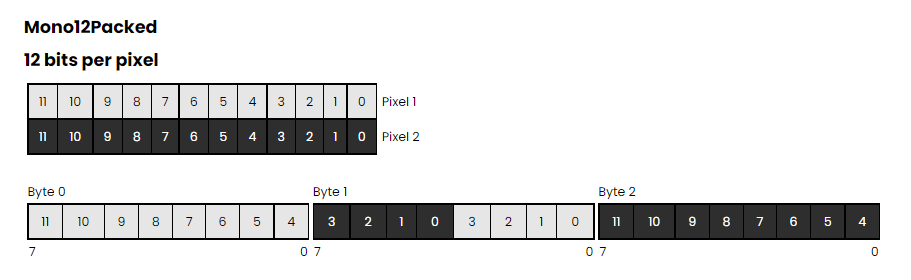
\includegraphics[width=\textwidth]{figures/polarized_image/Mono12Packed.png}
    \caption{Bit layout of the \cite{fisherRe15406LUT2023}}
    \label{fig:mono12packed}
\end{figure}




\begin{figure}
    \centering
    
\includegraphics[width=0.48\textwidth]{figures/unpacking/test_pattern0.jpg}
    
\includegraphics[width=0.48\textwidth]{figures/unpacking/test_pattern2.jpg}
    \caption{Test images used to identify bit pattern.}
\end{figure}

\begin{figure}
    \centering
    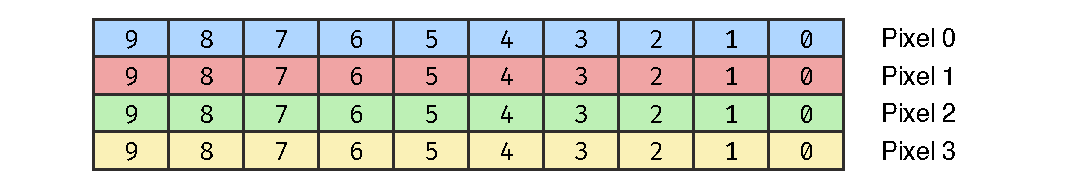
\includegraphics[width=\textwidth]{figures/unpacking/layout_10p.pdf}
    \caption{Bit layout of the \code{Mono10p} format.}
\end{figure}

\begin{figure}
    \centering
    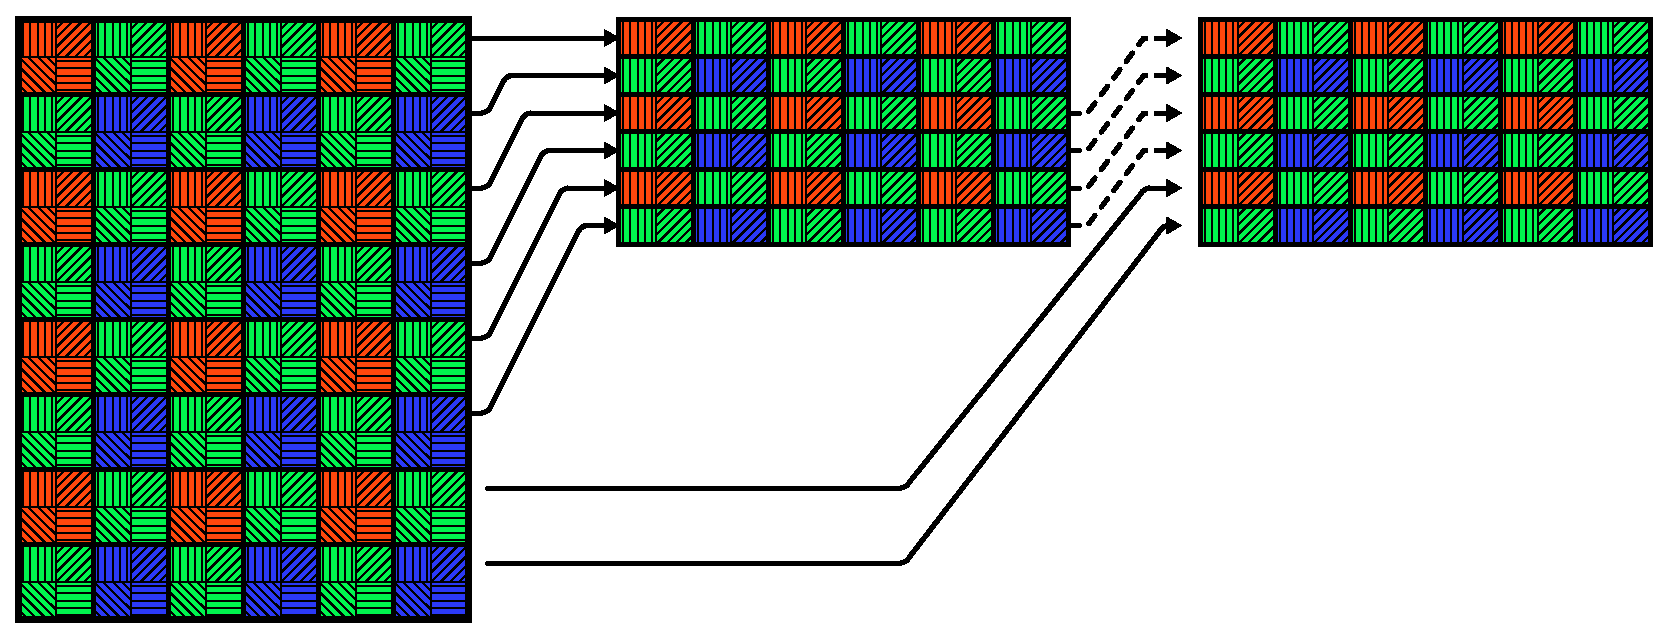
\includegraphics[width=\textwidth]{figures/polarized_image/read_line.pdf}
    \caption{TODO}
\end{figure}

\subsubsection{Contiguous acces using warp level primitives} \label{sec:contuguous_access}
As we want to operate on 32-bit values and each pixel is stored as a 10bit value, each thread is processing 160 bits, or five words as it is the lowest common multiple of 32 and 10.
Thus every thread reads five consecutive words as shown:
\begin{align}
    a_T[i] = d[T*32+i], &  & i \in (0,1,2,3,4)
\end{align}
Where $T$ is the thread intex in the warp, $a_T$ is local memory of thread $T$, $d$ is the image stored in device memory, and $k$ is some constant offset.

It was hypothized that it would be faster to let first read the data contiguously as and then redistribute the data as follows:
\begin{align}
    c_T[i] & = d[i*32+T],        &   &                 & i & \in (0,1,2,3,4) \\
    a_T[i] & = c_j[(T*5+i)//32], & j & = (T*5 + i)\%32 & i & \in (0,1,2,3,4)
    \label{eq:contiguous_reading}
\end{align}
Where $c_T$ is local memory of thread $T$ and $//$ is the ineger division operator, i.e. $x//y = \lfloor x/y \rfloor$.
The full table of all the values in a warp are shown in Table \ref{table:memory_index} in Appendix \ref{appendix:additional_resources}.

First it was attempted copy data from device memory into shared memory as shown in eq.\ref{eq:contiguous_reading}, but this turned out to be slower.
A secont attmempt was donw using the \code{__shfl_sync} function which is a warp-level primitive used to exchange data between threads in a warp \cite{linUsingCUDAWarpLevel2018}.
As the data exchange is performed directly between registers this is faster than going through shared memory \cite{linUsingCUDAWarpLevel2018}
However instead of specifiying what data to read from what thread, as in Eq. \ref{eq:contiguous_reading}, you need specity what data to send and what thread to read from, which is more difficult.
\begin{align}
    c_T[i] & = d[i*32+T],       &   &                 & i & \in (0,1,2,3,4) \\
    c_T[j] & \rightarrow a_x[i] & j & = \todo         & i & \in (0,1,2,3,4) \\
    a_T[i] & \leftarrow c_j[x]  & j & = (T*5 + i)\%32 & i & \in (0,1,2,3,4)
    \label{eq:contiguous_reading}
\end{align}
Where $x$ represents some locally unknown variable.

\todo cache stuff test


\begin{listing}[H]
    \begin{minted}{cuda}
        template <int width, int width_in>
        __device__ __forceinline__ void unpack10(__half2 *work_row, 
                                                 const unsigned int *img_row,
                                                 int tx) {
            __half2 *const out = &work_row[tx * 8 + 2];
        
            if (tx * 5 < width_in) {
                unsigned int buf_a, buf_b;
                buf_a = img_row[tx * 5];
                buf_b = img_row[tx * 5 + 1];
                out[0] = __halves2half2(buf_a & 0b1111111111, 
                                        buf_a >> 10 & 0b1111111111);
                out[1] = __halves2half2(buf_a >> 20 & 0b1111111111,
                                        buf_a >> 30 & 0b11 | (buf_b & 0b11111111) << 2);
        
                buf_a = img_row[tx * 5 + 2];
                out[2] = __halves2half2(buf_b >> 8 & 0b1111111111, 
                                        buf_b >> 18 & 0b1111111111);
                out[3] = __halves2half2(buf_b >> 28 & 0b1111 | (buf_a & 0b111111) << 4,
                                        buf_a >> 6 & 0b1111111111);

                buf_b = img_row[tx * 5 + 3];
                out[4] = __halves2half2(buf_a >> 16 & 0b1111111111,
                                        buf_a >> 26 & 0b111111 | (buf_b & 0b1111) << 6);
                out[5] = __halves2half2(buf_b >> 4 & 0b1111111111, 
                                        buf_b >> 14 & 0b1111111111);
        
                buf_a = img_row[tx * 5 + 4];
                out[6] = __halves2half2(buf_b >> 24 & 0b11111111 | (buf_a & 0b11) << 8,
                                        buf_a >> 2 & 0b1111111111);
                out[7] = __halves2half2(buf_a >> 12 & 0b1111111111, 
                                        buf_a >> 22 & 0b1111111111);
            }
            if (tx < 2) {
                work_row[tx] = work_row[tx + 2];
            } else if (tx >= width - 2 && tx < width) {
                work_row[tx + 4] = work_row[tx + 2];
            }
        }
    \end{minted}
    \caption{Bit unpacking in \cuda}
\end{listing}